\documentclass{article}
\usepackage[left=0cm,top=0cm,right=0cm,bottom=0cm]{geometry}
\setlength \paperwidth{6. true cm}
\setlength \paperheight{9 true cm}
\setlength \unitlength{1 true cm}
\usepackage{graphicx}
\usepackage{subfig}
\begin{document}
\begin{picture}(6, 9)
\put(-0.5, 6.0){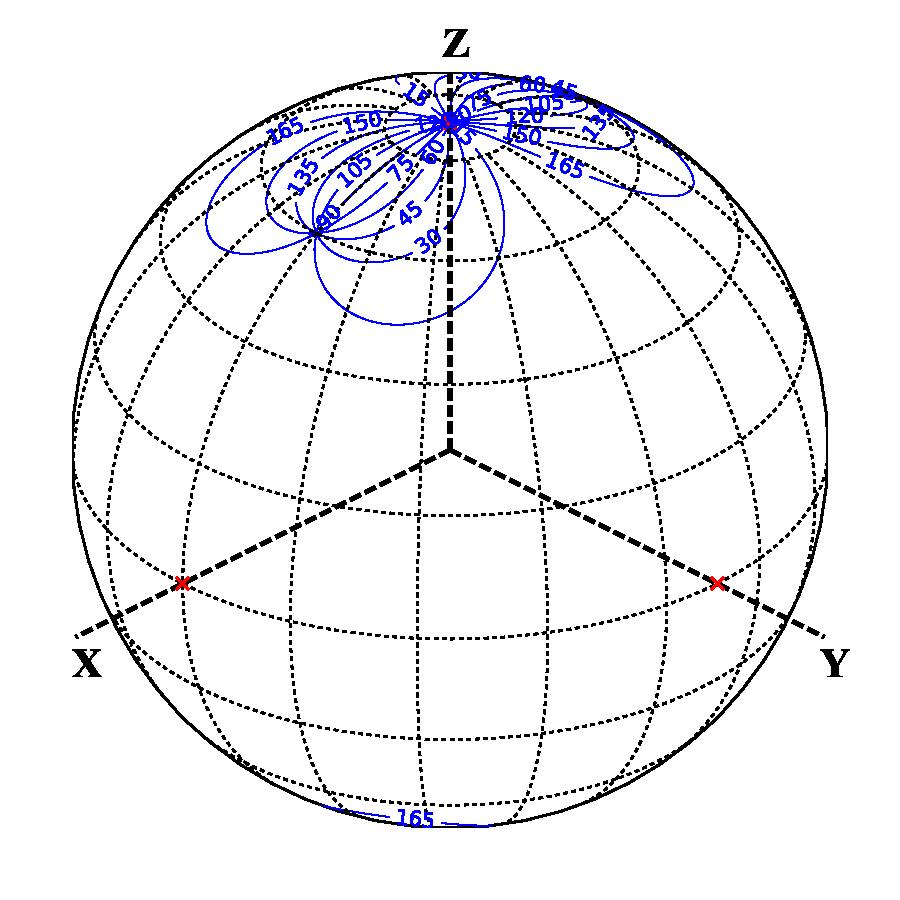
\includegraphics[width=3cm]{Gamma_min-A.pdf}}
\put(2.5, 6.0){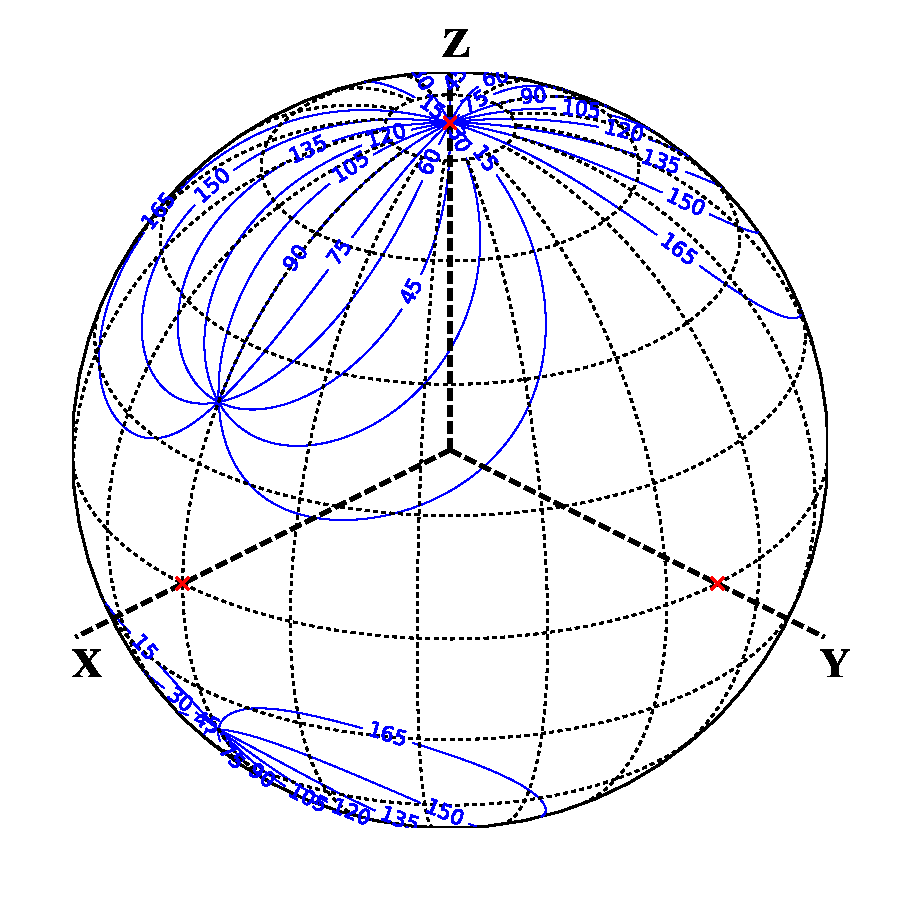
\includegraphics[width=3cm]{Gamma_min-B.pdf}}
\put(-0.5, 3.0){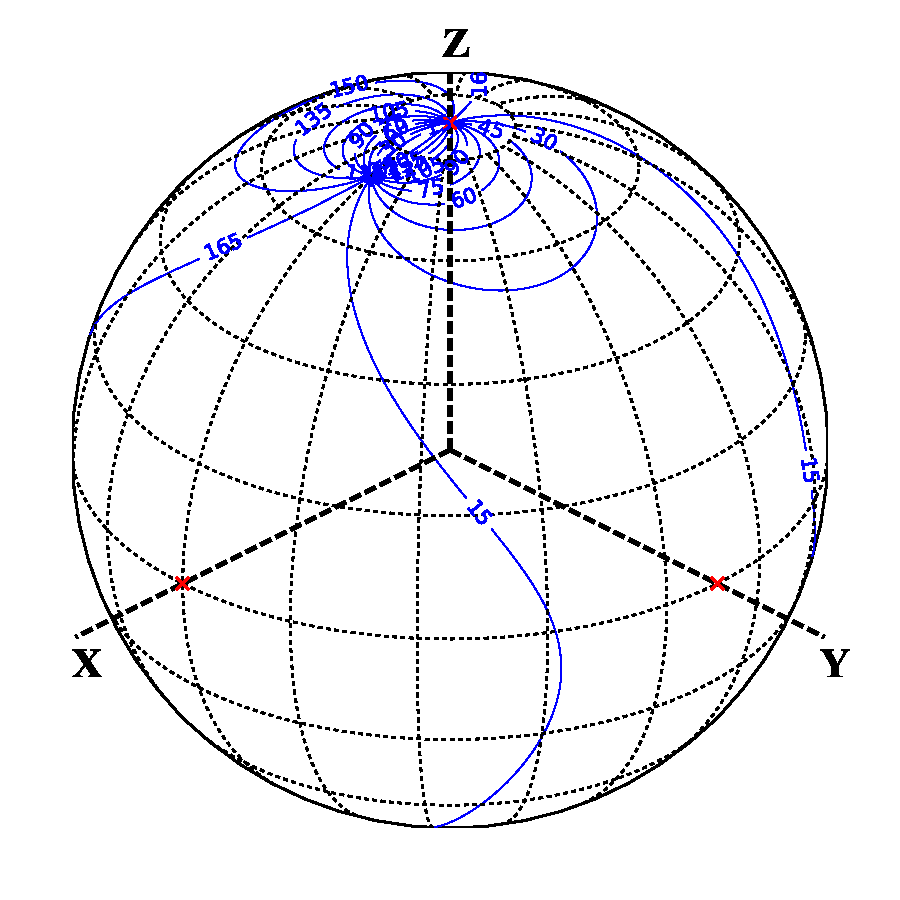
\includegraphics[width=3cm]{Gamma_kin-A.pdf}}
\put(2.5, 3.0){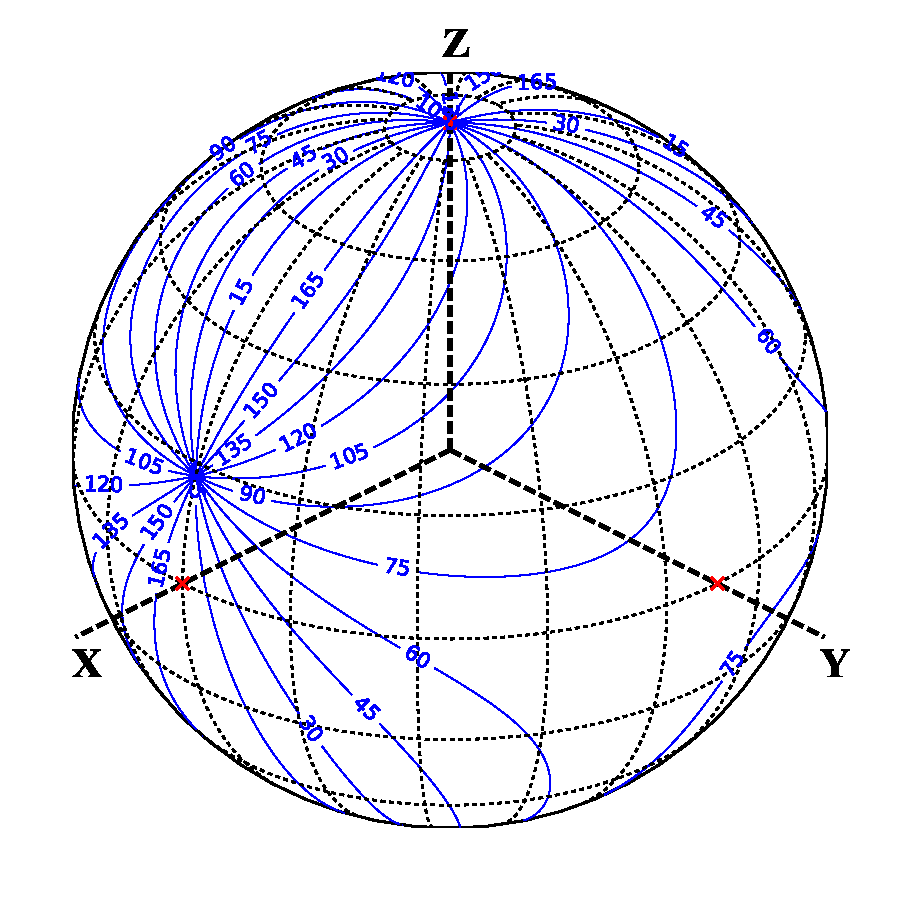
\includegraphics[width=3cm]{Gamma_kin-B.pdf}}
\put(-0.5, 0.0){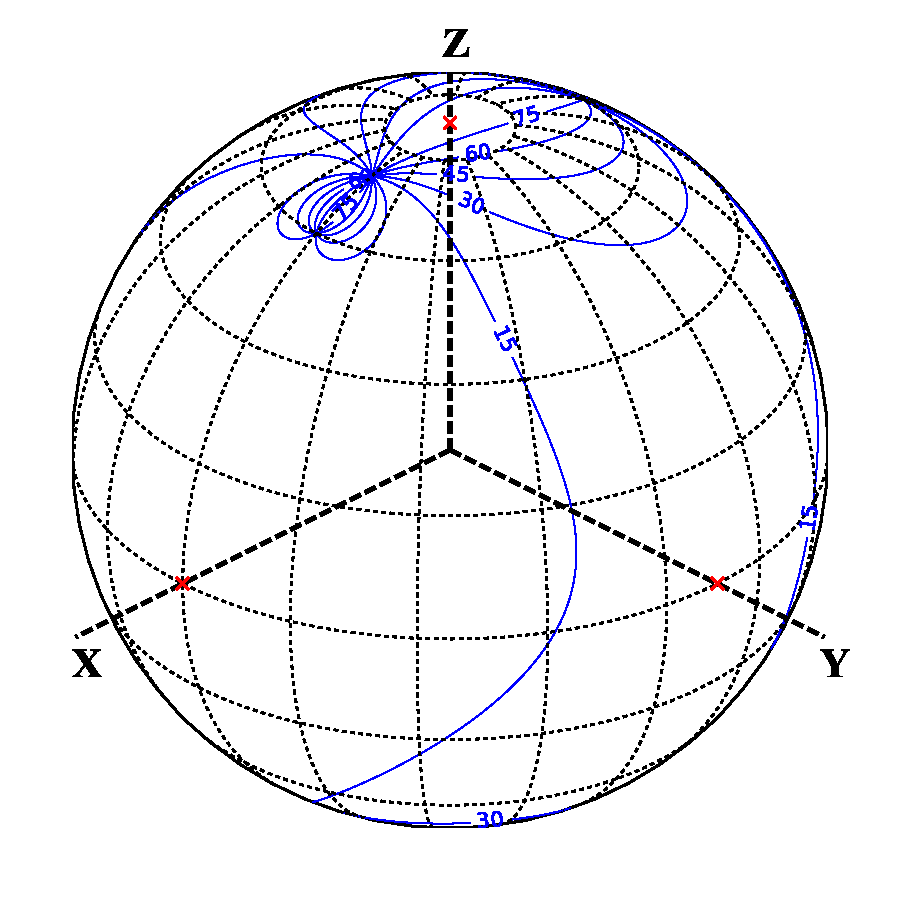
\includegraphics[width=3cm]{Psai-A.pdf}}
\put(2.5, 0.0){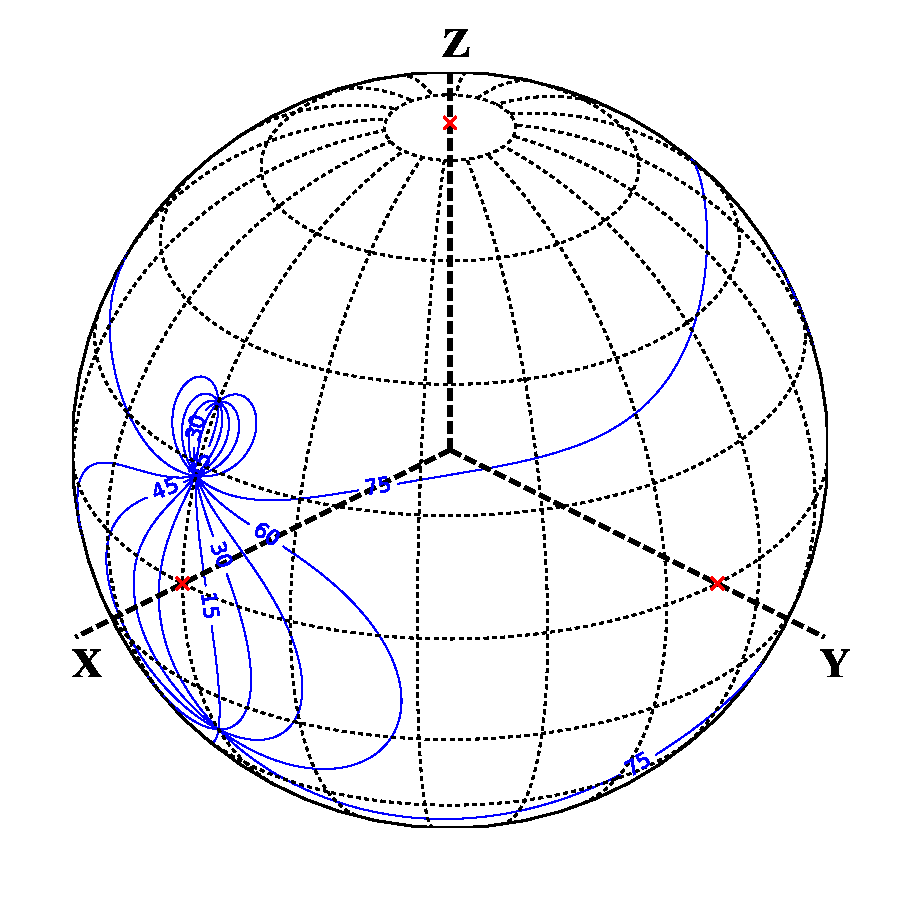
\includegraphics[width=3cm]{Psai-B.pdf}}
\end{picture}
\end{document}
